\documentclass[aps,%
14pt,%
final,%
oneside,
onecolumn,%
musixtex, %
superscriptaddress,%
centertags]{extarticle} %% 
\usepackage[english,russian]{babel}
\usepackage[utf8]{inputenc}
%всякие настройки по желанию%
\usepackage[colorlinks=true,linkcolor=blue,unicode=true]{hyperref}
\usepackage{euscript}

\usepackage{algorithm}
\usepackage{algpseudocode} 
\usepackage{supertabular}
\usepackage[pdftex]{graphicx}
\usepackage{amsthm,amssymb, amsmath}
\usepackage{textcomp}
\usepackage[bottom=20mm, top=20mm, left=30mm, right=15mm]{geometry}
\usepackage[usenames, dvipsnames]{color}
\usepackage{comment}

\makeatletter
\renewcommand{\ALG@name}{Листинг}
%\def\algorithmicwhile{\textbf{до тех пор, пока}}
\def\algorithmicrequire{\textbf{Вход:}}
\def\algorithmicensure{\textbf{Выход:}}
\def\algorithmicforall{\textbf{Для всех}}
\def\algorithmicdo{\textbf{}}
\def\algorithmicend{\textbf{Конец цикла}}
\def\algorithmicfor{\textbf{}}
\renewcommand{\algorithmicif}{\textbf{si}}%
%\renewcommand{\algorithmicthen}{\textbf{alors}}%
%\renewcommand{\algorithmicreturn}{\textbf{fin}}%

\DeclareMathOperator*{\argmin}{argmin}
\DeclareMathOperator*{\argmax}{argmax} 

\usepackage{graphicx}
\begin{document}

\begin{titlepage} 
\begin{center}
% Upper part of the page
{\large САНКТ-ПЕТЕРБУРГСКИЙ \\ ГОСУДАРСТВЕННЫЙ УНИВЕРСИТЕТ} \\[1.0cm]
{\large Математическое обеспечение и администрирование информационных систем} \\[0.2cm]
{\large Кафедра системного программирования} \\[3.5cm]
 
% Title
\textbf{\Large Назаренко Владимир Владимирович} \\[1cm]
\textbf{\LARGE Выделение объектов}\\[2mm]
\textbf{\LARGE на видеопоследовательности}\\[1.0cm]
{\Large Выпускная квалификационная работа} \\[3.5cm]

%supervisor
\begin{flushright} \large
\emph{Научный руководитель:} \\
ст. преп. \textsc{Смирнов М. Н.}
\end{flushright}
 \begin{flushright} \large
\emph{Рецензент:} \\
\textsc{Пенкрат Н. А.} \\
менеджер проектов, ООО ``Ланит-Терком''
\end{flushright}
\vfill 

% Bottom of the page
{\large {Санкт-Петербург}} \\[2mm]
{\large {2018 г.}}
\end{center} 
\end{titlepage}

\begin{titlepage} 
\begin{center}
% Upper part of the page
{\large SAINT PETERSBURG STATE UNIVERSITY} \\[1.0cm]
{\large Software and Administration of Information Systems} \\[0.2cm]
{\large Software Engineering Department} \\[3.5cm]
 
% Title
\textbf{\Large Vladimir Nazarenko} \\[1cm]
\textbf{\LARGE Object detection in a video sequence}\\[1.0cm]
{\Large Master thesis} \\[3.5cm]

%supervisor
\begin{flushright} \large
\emph{Scientific advisor:} \\
sr. Lecturer \textsc{Mikhail Smirnov}
\end{flushright}
 \begin{flushright} \large
\emph{Reviewer:} \\
\textsc{Nickolay Penkrat} \\
Project Manager, Lanit-Tercom LLC
\end{flushright}
\vfill 

% Bottom of the page
{\large {St Petersburg}} \\[2mm]
{\large {2018}}
\end{center} 
\end{titlepage}

\tableofcontents

\setcounter{page}{3}

\newpage

\section*{Введение}

На автомобильных дорогах происходит большое количество дорожно - транспортных происшествий (ДТП). Согласно исследованию \cite{staubach2009factors} причиной большого количества ДТП является водитель, внимательность которого ослаблена в следствие усталости, приёма медицинских препаратов, имеющих седативный эффект, алкогольного опьянения, выполнения задач, не связанных с управлением транспортным средством и др.

В настоящее время широкое распространение получили системы помощи водителю\cite{Shaout2011AdvancedDA}. Такие системы, например, предупреждают водителя об ограничении скорости на участке дороге (с помощью распознавания соответствующих дорожных знаков), о пересечении маркеров дорожной разметки, об опасности столкновения с различными объектами\cite{lu2005technical}. Существуют исследования, экспериментально доказывающие практическую полезность таких систем \cite{maag2012studying}.

Важным элементом таких систем являются различные сенсоры. Наиболее распространёнными сенсорами для решения перечисленных выше задача являются лидары, радары, ультразвуковые датчики и оптические системы видимого спектра (стерео- и монокамеры). Область применения каждого из типов сенсоров ограничена\cite{lu2005technical}\cite{ziebinski2016survey}. Так, радары обладают низкой точностью определения формы и расстояния до объекта. Лидары обладают низкой точность в плохих погодных условиях. Кроме того, высокая стоимость лидаров делает решения на их основе недоступными для массового сегмента автомобильной промышленности. Ультразвуковые датчики способны обнаруживать препятствия только на небольших расстояниях. Использование оптических систем требует использования сложных для определения расстояния до объектов. 

Стереокамера сочетает в себе невысокую стоимость, возможность с высокой точностью определять геометрию и расстояние до объектов, простоту монтажа.


На кафедре системного программирования Санкт-Петербургского государственного университета в совместных исследовательских проектах с компанией Prosense (Южная Корея), разрабатываются алгоритмы для системы помощи водителю. Одним из требований к этой системе является низкая стоимость и возможность установки системы без существенных модификаций конструкции автомобиля. Одной из частей этой системы является так называемый \textit{\textbf{сенсор безопасного движения}} -- подсистема, предупреждающая водителя о потенциальных столкновениях и пересечении маркеров дорожной разметки.

В данной работе мы сфокусировались на разработке и апробации алгоритмов для сенсора безопасного движения. В связи с требованиями к разрабатываемой системе, а именно, ограничением на стоимость и простоту монтажа, в качестве сенсора мы выбрали стереокамеру, состоящую из двух откалиброванных камер видимого диапазона.

Существует, как минимум, два класса алгоритмов для решения задач помощи водителю, использующих оптические сенсоры: нейросетевые алгоритмы и алгоритмы на основе методов классического компьютерного зрения. В данной работе было решено использовать алгоритмы на основе классического компьютерного зрения. Связано это со следующими проблемами нейросетевых алгоритмов.\cite{lipton2016mythos}
\begin{itemize}
\item Сложность модификации нейросетевых алгоритмов.
\item Неуниверсальность нейросетевых алгоритмов.
\item Сложность интерпретации решений нейросетевых алгоритмов.
\end{itemize}

 Строго говоря, под предупреждением водителя о потенциальном столкновении мы понимаем детектирование на изображении \textit{\textbf{препятствий}} -- любых объектов, которые делают невозможным или опасным проезд через занимаемую ими область пространства. Типовыми примерами препятствий являются люди, автомобили, столбы, здания. Также мы считаем препятствиями особенности рельефа (холмы) и различные мелкие объекты, такие как бордюры. Слова ``объект'' и ``препятствие'' для нас являются синонимами. Под \textit{\textbf{детектированием препятствий}} мы понимаем выделение препятствий на изображении в том или ином виде. Например, в виде описывающего прямоугольника или в виде области на изображении, движение в которой безопасно -- \textit{\textbf{безопасной области}}.

Также отметим, что термины ``выделение объектов'', ``детектирование объектов'' и ``сегментация изображения на объекты'' мы считаем эквивалентными.

Под \textit{\textbf{детектированием маркеров дорожной разметки}} мы понимаем задачу выделения на изображении таких маркеров, как одиночная сплошная линия, двойная сплошная линия, прерывистая линия, бордюры.

\newpage
\section{Постановка задачи}

Целью данной работы является разработка и реализация, на основе подходов классического стерео-зрения и классической обработки изображений, алгоритмов для ``сенсора безопасного движения''.
Для достижения этой цели в рамках работы были сформулированы следующие задачи.
\begin{itemize}
    \item Разработать и реализовать прототип алгоритма поиска препятствий движению автомобиля на изображении, полученном с помощью стереокамеры.
    \item Разработать и реализовать прототип алгоритма поиска маркеров дорожной разметки на изображении, полученном с помощью стереокамеры.
    \item Провести апробацию разработанных алгоритмов.
\end{itemize}

\newpage
\section{Обзор}

\subsection{Основные определения}

Единственным сенсором, который мы используем для решения поставленных задач является стереокамера.

\textbf{\textit{Стереокамера}} это система из двух камер, расположенных на небольшом расстоянии друг от друга, взаимное расположение и калибровка которых известны в любой момент времени. Ключевым свойством такой системы является возможность оценки расстояния до объектов на изображении за счёт параллакса.

\textbf{\textit{Оптический поток}} -- это отображение пикселей изображения в пару целочисленных значений, соответствующих движению объекта реального мира, спроецированного в пиксель, в плоскости камеры.

С использованием стереокамеры становится возможным вычислить \textbf{\textit{карту глубины}} -- отображение, сопоставляющее пикселю исходного изображения расстояние от оптического центра камеры до точки в пространстве, которая была спроецирована в данный пиксель. Карта глубины может быть плотной, в таком случае подразумевается, что большинству пикселей сопоставлено значение глубины, либо неплотной -- значение глубины сопоставлено лишь некоторым пикселям. В случае неплотной карты глубины, как правило, значения глубины сопоставлены так называемым ключевым точкам -- точкам, в которых на изображении имеется выраженный перепад яркостей.

В настоящее время алгоритмы построения карты глубины используют \textbf{\textit{ректифицированные изображения}} -- это пара изображений, к которым применено перспективное преобразование, модифицирующее исходную пару изображений, симулируя расположение плоскостей обеих камер в одной и той же плоскости.

Основным шагом вычисления карты глубины является вычисление диспаритета для каждого пикселя. \textbf{\textit{Диспаритет}} это смещение между координатами пикселя, соответствующего одной и той же точке пространства на первом и втором сенсорах стереокамеры. Как правило, диспаритет вычисляется для пары ректифицированнх изображений. В таком случае диспаритет -- это одно число, смещение по горизонтальной оси. В тексте данной работы в некоторых местах мы взаимозаменяемо употребляем термины ``карта диспаритетов'' и ``карта глубины''. Связано это с тем, что переход от одной карты к другой в нашем случае возможно осуществить путём домножения на константу.

\subsection{Карта глубины}

Построение карты глубины является популярным методом предобработки пары изображений, полученных с помощью стереокамеры, и используется во многих работах, авторы которых решают задачу детектирования препятствий.

Существуют альтернативные методы предобработки для вычисления геометрии и расстояния до объектов на изображении \cite{monodepth17}\cite{koenderink1991affine}, основанные на использовании одной камеры, однако они проигрывают построению карты глубины по снимку, полученному с помощью стереокамеры либо в точности, либо в качестве результатов. Поэтому в данной работе мы придерживаемся подхода на основе построения карты глубины.

Способ построения карты глубины критически важен для алгоритма детектирования препятствий, разработанного в рамках данной работы. Различные алгоритмы отличаются друг от друга как качеством, так и скоростью работы. Разработка собственного алгоритма построения карты глубины находится за пределами данной работы, однако нами были рассмотрены следующие реализации алгоритмов.
\begin{itemize}
\item Реализация алгоритма Semi-global Matching из открытой библиотеки компьютерного зрения OpenCV\cite{itseez2015opencv}.
\item Закрытая реализация алгоритма AD-Census.
\item Закрытая реализация алгоритма вычисления разреженной карты глубины CVS.
\end{itemize}

\subsubsection{Алгоритм Semi-global Matching}
Алгоритм Semi-global Matching \cite{hirschmuller2005accurate} (SGM) широко применяется для вычисления карты глубины.

Данный алгоритм минимизирует целевую функцию, заданную в выражении \ref{eq:sgm_cost} на паре ректифицированных изображений, полученных с помощью стереокамеры.

\begin{equation} \label{eq:sgm_cost}
E(D)=\sum_p [C(p, D_p) + \sum_{q \in N_p \land |D_p - D_q| = 1} P_1 + \sum_{q \in N_p \land |D_p - D_q| > 1} P_2]
\end{equation}

Здесь $p$ это координаты пикселя на левом изображении, $C(p, D_p)$ -- значение функции схожести левого и правого изображения стереокамеры, $P_1$ и $P_2$ -- константные штрафы, $N_p$ -- окрестность точки $p$ на левом изображении, $D_p$ и $D_q$ -- значения диспаритетов для пикселей $p$ и $q$.

Особенностью алгоритма SGM является то, что минимизация целевой функции производится сразу по нескольким направлениям, как это изображено на рисунке \ref{fig:sgm_paths}.

\begin{figure}[htp]
\centering
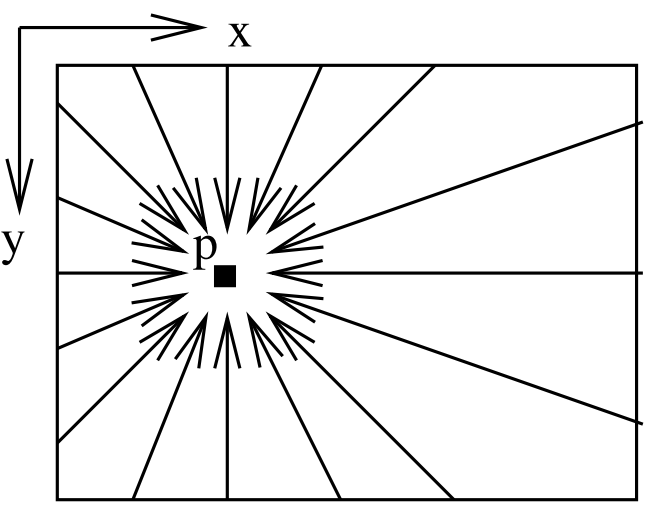
\includegraphics[scale=0.3]{sgm_paths.png}
\caption{Схема направлений оптимизации в алгоритме SGM \cite{hirschmuller2005accurate}}
\label{fig:sgm_paths}
\end{figure}

В целях предобработки пары изображений, полученных с помощью стереокамеры, нами была использована общедоступная реализация алгоритма SGM из открытой библиотеки OpenCV. В данной реализации в качестве функции схожести $C(p, D_p)$ используется сумма абсолютных разниц (SAD) в окрестности пикселя.

\subsubsection{Алгоритм AD-Census}
Алгоритм AD-Census \cite{mei2011building} является модификацией алгоритма SGM для систем массового параллелизма, таких как графические ускорители.

В отличие от алгоритма SGM, в алгоритме AD-Census используется функция схожести, основанная на взвешенном среднем двух компонент: абсолютной разности интенсивностей (компонента AD) и расстоянии Хэмминга (компонента Census). Кроме того, авторы предлагают ряд модификаций оригинального алгоритма SGM для практического уменьшения количества требуемых вычислений.

В целях предобработки пары изображений, полученных с помощью стереокамеры, нами была использована закрытая реализация алгоритма AD-Census, выполненная инженерами компании Ланит-Терком.


\subsubsection{Алгоритм CVS}
Алгоритм CVS является запатентованной разработкой компании Ланит-Терком. Данный алгоритм позволяет строить разреженную карту глубины, где значения глубины сопоставляются ключевым точкам -- пикселям на изображении, соответствующим выраженным перепадам яркости на изображении.

\textbf{\Large \color{Red} TODO: Цитировать статью или патент}

\subsubsection{Сравнение алгоритмов построения карты глубины}

\textbf{\Large \color{Red} TODO: Изображение -- качественное сравнение алгоритмов расчёта карты глубины}

\subsection{Существующие подходы к детектированию препятствий с помощью стереокамеры}

Существует большое количество исследований в области детектирования неклассифицированных объектов с помощью стереокамеры. В рамках работы было проведено изучение соответствующих работ. Перечислим далее работы, наиболее  релевантные нашей цели.

Авторы \cite{heinrich2002fast} предложили использовать геометрическую зависимость между оптическим потоком и расстоянием до объекта, вычисленным с помощью алгоритмов построения карты глубины. Как отмечают авторы, данный подход неустойчив к движению камер в плоскости кадра и к неточностям алгоритмов расчёта оптического потока и карты глубины. К плюсам предложенного решения можно отнести высокую скорость работы, без учёта вычисления оптического потока и расчёта карты глубины.

В работе \cite{labayrade2002real} авторы представили способ определения рельефа дорожной поверхности без использования карты глубины. Также авторы показали принципиальную возможность выделять отдельные препятствия с помощью представленного ими алгоритма. Однако точность алгоритма невысока, особенно в случае наличия большого количества препятствий на изображении. Тем не менее, способ динамического определения положения дорожного полотна, предложенный в этой работе, широко используется. В том числе, он был использован в нашем исследовании.

Развивая подход Labayrade \cite{labayrade2002real}, авторы \cite{broggi2006single} предлагают улучшения для алгоритма, позволяющие применять алгоритм в ситуациях бездорожья. Тем не менее авторы приводят только качественную оценку своего алгоритма, из которой следует вывод, что алгоритм применим только в ситуациях с небольшим количеством препятствий на изображении, как и подход Labayrade  \cite{labayrade2002real}.

В работе \cite{franke20056d} предложен подход выделения препятствий на изображении, основанный на расчёте неплотного оптического потока с помощью KLT-трекера и фильтра Калмана и расчёте неплотной карты глубины. Авторы данной работы не приводят способа выделения отдельных объектов на изображении, также в данной работе не рассмотрено выделение препятствий, не имеющих собственного движения.

В статье \cite{pfeiffer2010efficient} авторы предлагают вместо вычисления карты глубины сегментировать изображение на вертикальные полосы, для каждой из которых вычисляются две горизонтальных границы, соответствующие основанию ближайшего препятствия и его высоте. Затем, используя эту сегментацию, можно выделить объекты не прибегая к сложным вычислениям. Данный подход показался нам перспективным и многие идеи нашего исследования были заимствованы из данной работы, поэтому опишем этот алгоритм подробно.


\subsection{Динамическое определение положения плоскости дорожного полотна}\label{vdisparity_explanation}

В данной работе мы использовали оценку плоскости дорожного полотна с помощью алгоритма, предложенного в статье \cite{labayrade2002real}. Авторы предлагают для каждой строки карты диспаритетов построить гистограмму, затем получившиеся гистограммы сконкатенировать. Получившееся изображение авторы носит название ``vdiparity image''. На изображении \ref{fig:vdisp_example} приведён пример вычисления плоскости дорожного полотна. Слева направо на этом изображении представлены фрагмент исходного левого изображения, ``vdisparity image'', ``vdisparity image``, на котором пунктирной линией отмечена область, соответствующая диспаритету дороги. Поиск этой области осуществляется наложением на модель параметрической модели (в данном случае, линии), с помощью преобразования Хафа. Получившаяся линия имеет следующую интерпретацию: если точка с координатами $(x, y)$ принадлежит линии, то ожидаемое значение диспаритета плоскости дороги в строке изображения $y$ равно $x$.

\begin{figure}[htp]
\centering
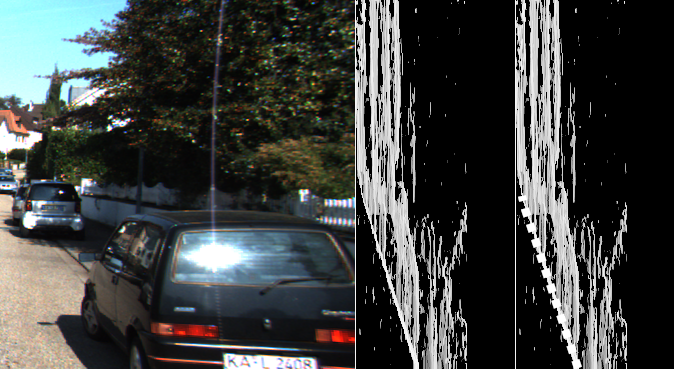
\includegraphics[width=\textwidth]{vdisp_concat.png}
\caption{Пример определения плоскости дорожного полотна}
\label{fig:vdisp_example}
\end{figure}

\subsection{Подход Stixel World} \label{sec:stixels}

Опишем подход, предложенный в статье \cite{pfeiffer2010efficient}, подробнее, так как наша работа основана на данном подходе.

\begin{figure}[htp]
\centering
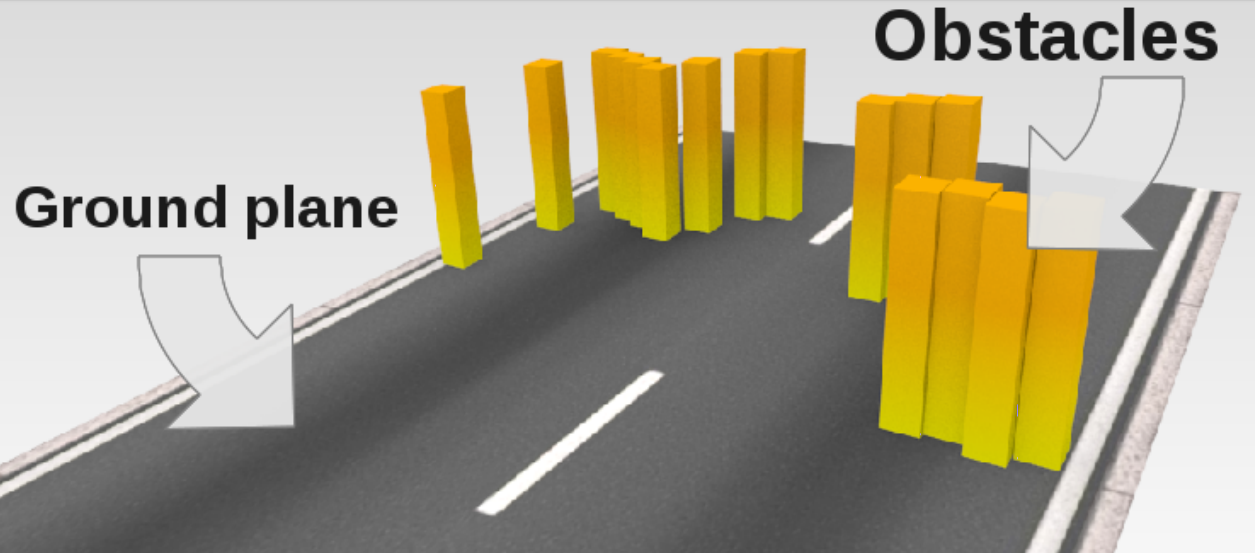
\includegraphics[width=\textwidth]{stixels_basic.png}
\caption{Упрощённое представление мира в модели Stixel World \cite{benenson2011stixels}}
\label{stixels_basic}
\end{figure}

В модели Stixel World препятствия описываются упрощённой моделью: предполагается, что любое препятствие может быть хорошо приближено параллелепипедом. В таком случае на изображении препятствия могут быть хорошо приближены набором вертикальных прямоугольников с сопоставленными им значениями глубины. На рис. \ref{stixels_basic} изображена схема упрощённой модели препятствий, принятой в модели Stixel World.

Таким образом, модель Stixel World предполагает сегментацию изображения на стиксели -- прямоугольники фиксированной ширины. Каждому стикселю соответствует 4 следующих значения.
\begin{enumerate}
\item Индекс стикселя.
\item Координата строки изображения -- нижняя граница стикселя. 
\item Координата строки изображения -- верхняя граница стикселя.
\item Значение расстояния. При этом предполагается, что расстояние одинаково до всех пикселей, принадлежащих стикселю.
\end{enumerate}

Пример сегментации изображения, получаемый с использованием модели Stixel World, представлен на рис. \ref{stixels_segm}.

\begin{figure}[htp]
\centering
\includegraphics[width=\textwidth]{/home/me/mm/master/stixels_example.png}
\caption{Пример сегментации препятствий с помощью стикселей. Цветом закодировано расстояние.}
\label{stixels_segm}
\end{figure}

Для построения модели Stixel World по двум изображениям, полученным с помощью стереокамеры, авторы предлагают минимизировать сумму двух целевых функций.

\begin{equation}\label{eq:stix_basic}
d^*_s(u) = \argmin_{d(u)}\sum_u c_s(u, d(u)) + \sum_{u_a, u_b} s_s(d(u_a), d(u_b))
\end{equation}

\begin{equation}
c_s(u, d) = c_o(u, d) + c_g(u, d)
\end{equation}

\begin{equation}\label{eq:stix_co}
c_o(u, d) = \sum_{v=v(h_o, d)}^{v(d)} c_m(u, v, d)
\end{equation}

\begin{equation}\label{eq:stix_cg}
c_g(u, d) = \sum_{v=v(d)}^{|V|} c_m(u, v, f_{ground}(v))
\end{equation}

\begin{equation}\label{eq:stix_ss}
s_s(d_a, d_b)=
\begin{cases}
  \infty, & \text{если}\ d_a < d_b - 1 \\
  c_o(u_a, d_a) & \text{если}\ d_a = d_b - 1 \\
  0, & \text{если}\ d_a > d_b - 1 \\
\end{cases}
\end{equation}

В формулах \ref{eq:stix_basic} -- \ref{eq:stix_ss} приняты следующие обозначения.

$u$ -- порядковый номер стикселя.

$v$ -- индекс строки изображения.

$d^*_s$ -- вычисленное значение диспаритета для стикселя под номером $u$.

$h_0$ -- минимальная высота объекта на сцене, в метрах.

$c_m(u, v, d)$ -- значение функции схожести в точке $(u, v)$ для диспаритета $d$.

$f_{ground}(v)$ -- диспаритет плоскости дороги для строки $v$ изображения.

$u_a, u_b$ -- индексы соседних стикселей.

Также авторы предлагают способ оценки высоты объектов с помощью оценки высоты стикселей. Для этого вводится схожая целевая функция, которую мы опустим для краткости.

Такая целевая функция допускает минимизацию на ректифицированной паре изображений с помощью техник динамического программирования, что и было предложено авторами модели Stixel World.

Данный подход требует значительно больше вычислительных ресурсов, в отличие от предыдущих, однако авторы \cite{benenson2011stixels} сообщают, что алгоритм может быть оптимизирован для работы в реальном времени.


\subsection{Подходы к детектированию маркеров дорожной разметки}

В рамках задачи детектирования маркеров дорожной разметки было проведено большое количество исследований\cite{hillel2014recent}. Множество подходов основано на методах глубокого обучения, однако мы отказались от таких методов в силу специфики задачи.

Альтернативой являются подходы на основе классического компьютерного зрения и параметрических моделей. Простейшей параметрической моделью является прямая. Оказывается, что детектирования прямых достаточно в случае движения по автомагистралям\cite{hillel2014recent}.

Работы, связанные с параметрическими моделями, во многом схожи, поэтому здесь приведём только две наиболее релевантные. 

В работе \cite{song2017real} к изображению сначала применяется преобразование Bird's Eye View, проецирующее плоскость камеры на плоскость дороги, затем производится выделение выраженных горизонтальных линий и выделение в пространстве Хафа набора линий, соответствующих набору маркеров дорожной разметки.

В работе \cite{aly2008real} производятся аналогичные преобразования изображения, однако линии задаются более сложной моделью -- в виде кубических сплайнов. Подбор параметров такой модели осуществляется с помощью алгоритма RANSAC. Однако усложнение модели ведёт к увеличению количества шума.


\newpage
\section{Алгоритм поиска препятствий движению автомобиля}

В данном разделе описан предложенный и реализованный в виде прототипа алгоритм поиска препятствий с помощью стереокамеры. Основные идеи данного подхода взяты из модели Stixel World \cite{pfeiffer2010efficient}, описанной в разделе \ref{sec:stixels}.

В предлагаемом нами алгоритме мы, вслед за авторами работы \cite{pfeiffer2010efficient}, представляем сцену, видимую на паре изображений, полученных с помощью стереокамеры, в виде модели Stixel World. Однако, в отличие от \cite{pfeiffer2010efficient}, вычисление параметров модели происходит не на паре изображений, а на карте диспаритетов.

Это изменение ведёт к модификации целевой функции. В связи с тем, что расстояние до точек изображения уже вычислено, для построения модели Stixel World достаточно для каждого стикселя вычислить координаты верхней и нижней границ. Модифицированная целевая функция для оценки нижней границы стикселей имеет вид, описанный в формуле \ref{eq:mystix_basic}. Отметим, что размер левого изображения, правого изображения и карты диспаритетов мы считаем одинаковым.

В формулах \ref{eq:mystix_basic} -- \ref{eq:mystix_ss} принятны следующие обозначения, в целом соответствующие обозначениям раздела \ref{sec:stixels}.

$u$ -- индекс стикселя.

$v$ -- индекс строки изображения.

$v_{bot}(u)$ -- нижняя граница стикселя с индексом $u$.

$v_{bot}^*(u)$ -- оптимальная нижняя граница стикселя с индексом $u$.

$|V|$ -- количество строк изображения.

\begin{equation}\label{eq:mystix_basic}
v_{bot}^*(u) = \argmin_{v}[\sum_u c_s(u, v) + \sum_{u_a, u_b: |u_a - u_b| = 1} s_s(v_{bot}(u_a), v_{bot}(u_b))]
\end{equation}

Формула \ref{eq:mystix_basic} состоит из двух слагаемых. Первое слагаемое, $c_s(u, v)$, представляет собой оценку правдоподобности наличия нижней границы препятствия в строке $v$ стикселя $u$ и имеет вид, описанный в формулах \ref{eq:mystix_cost_bottom} -- \ref{eq:mystix_cg}. 

\begin{equation}\label{eq:mystix_cost_bottom}
c_s(u, v) = c_o(u, v) + c_g(u, v)
\end{equation}

\begin{equation}\label{eq:mystix_co}
c_o(u, v) = \sum_{v'=v(h_o, d(u, v))}^{v} |d(u, v) - d(u, v')|
\end{equation}

\begin{equation}\label{eq:mystix_cg}
c_g(u, v) = \sum_{v'=v}^{|V|} |d(u, v) - d_{ground}(u, v')|
\end{equation}

В формулах \ref{eq:mystix_cost_bottom} -- \ref{eq:mystix_cg} приняты следующие обозначения.

$c_o(u, v)$ -- функция правдоподобности наличия препятствия в стикселе $u$ на строке изображения $v$.

$c_g(u, v)$ -- функция правдоподобности отсутствия препятствия в стикселе $u$ в во всех строках изображения $v' : v' > v$.

$d_{ground}(u, v)$ -- ожидаемое значение диспаритета в стикселе $u$, в строке $u$ для плоскости дорожного полотна.

$d(u, v)$ -- медиана значений в строке $v$ карты диспаритетов, соответствующих стикселю $u$, т.е. медиана значений карты диспаритетов на позициях $(w * u, v)\dots (w * (u + 1) - 1, v)$, где $w$ -- предопределённая ширина стикселя.

Второе слагаемое формулы \ref{eq:mystix_basic} представлено в формуле \ref{eq:mystix_ss}. $c_{jump}$ в этой формуле обозначает наперёд заданный порог. В нашей реализации этот порог был принят равным $50$.

\begin{equation}\label{eq:mystix_ss}
s_s(v_a, v_b)=
\begin{cases}
  \infty,     & \text{если}\ |v_a - v_b| > c_{jump} \\
  |v_a - v_b| & \text{иначе}
\end{cases}
\end{equation}

Функция оценки верхней границы стикселей имеет схожий вид и представлена в формулах \ref{eq:mystix_height_basic} -- \ref{eq:mystix_cost_h}.

\begin{equation}\label{eq:mystix_height_basic}
v_{top}^*(u) = \argmin_{v}\sum_u c_s^h(u, v) + \sum_{v_{top}^a, v_{top}^b} s_s(v_{top}^a, v_{top}^b)
\end{equation}

\begin{equation}\label{eq:mystix_cost_h}
c_s^h(u, v) = \sum_{v'=v}^{v_{bot}} |d(u, v) - d(u, v')| - k * |d(u, v_{bot})| * |v' - v|
\end{equation}

Для вычисления функции \ref{eq:mystix_cg} требуется знание диспаритета плоскости дорожного полотна в стикселе $u$ в строке $v$. Для этого мы используем подход, предложенный в статье \cite{labayrade2002real} и описанный в разделе \ref{vdisparity_explanation}.

В листинге \ref{alg:stixels} представлен псевдокод алгоритма сегментации карты диспаритетов согласно модели Stixel World.

На иллюстрациях \ref{fig:stix_small} и \ref{fig:stix_offroad} приведены примеры работы алгоритма в двух режимах. На рис. \ref{fig:stix_small} алгоритм применён для детектирования небольшого объекта (детской игрушки), на рис. \ref{fig:stix_offroad} верхняя граница стикселей не показана, вместо этого выделена область, ограниченная нижней границей изображения и нижней границей стикселей.



\begin{algorithm}[H]
\caption{Сегментация карты диспаритетов согласно модели Stixel World}
\label{alg:stixels}
\begin{algorithmic}[1]
\Require Карта диспаритетов, ширина стикселя
\Ensure Множество стикселей, описывающих карту глубины согласно модели Stixel World
\State Вычислить значение $d_{ground}(u, v)$, используя алгоритм из раздела \ref{vdisparity_explanation}
\ForAll{$(u, v)$}
\State Вычислить значение $c_s(u, v)$, заданное функцией \ref{eq:mystix_cost_bottom}
\EndFor
\State С помощью динамического программирования минимизировать вычислить значения $v_{bot}^*(u_1) \dots v_{bot}^*(u_n)$, заданные функцией \ref{eq:mystix_basic}
\ForAll{$(u, v)$}
\State Вычислить значение $c_s^h(u, v)$, заданное функцией \ref{eq:mystix_cost_h}
\EndFor
\State С помощью динамического программирования вычислить значения $v_{top}^*(u_1) \dots v_{top}^*(u_n)$, заданные функцией \ref{eq:mystix_height_basic}
\end{algorithmic}
\end{algorithm}

\begin{figure}[H]
\centering
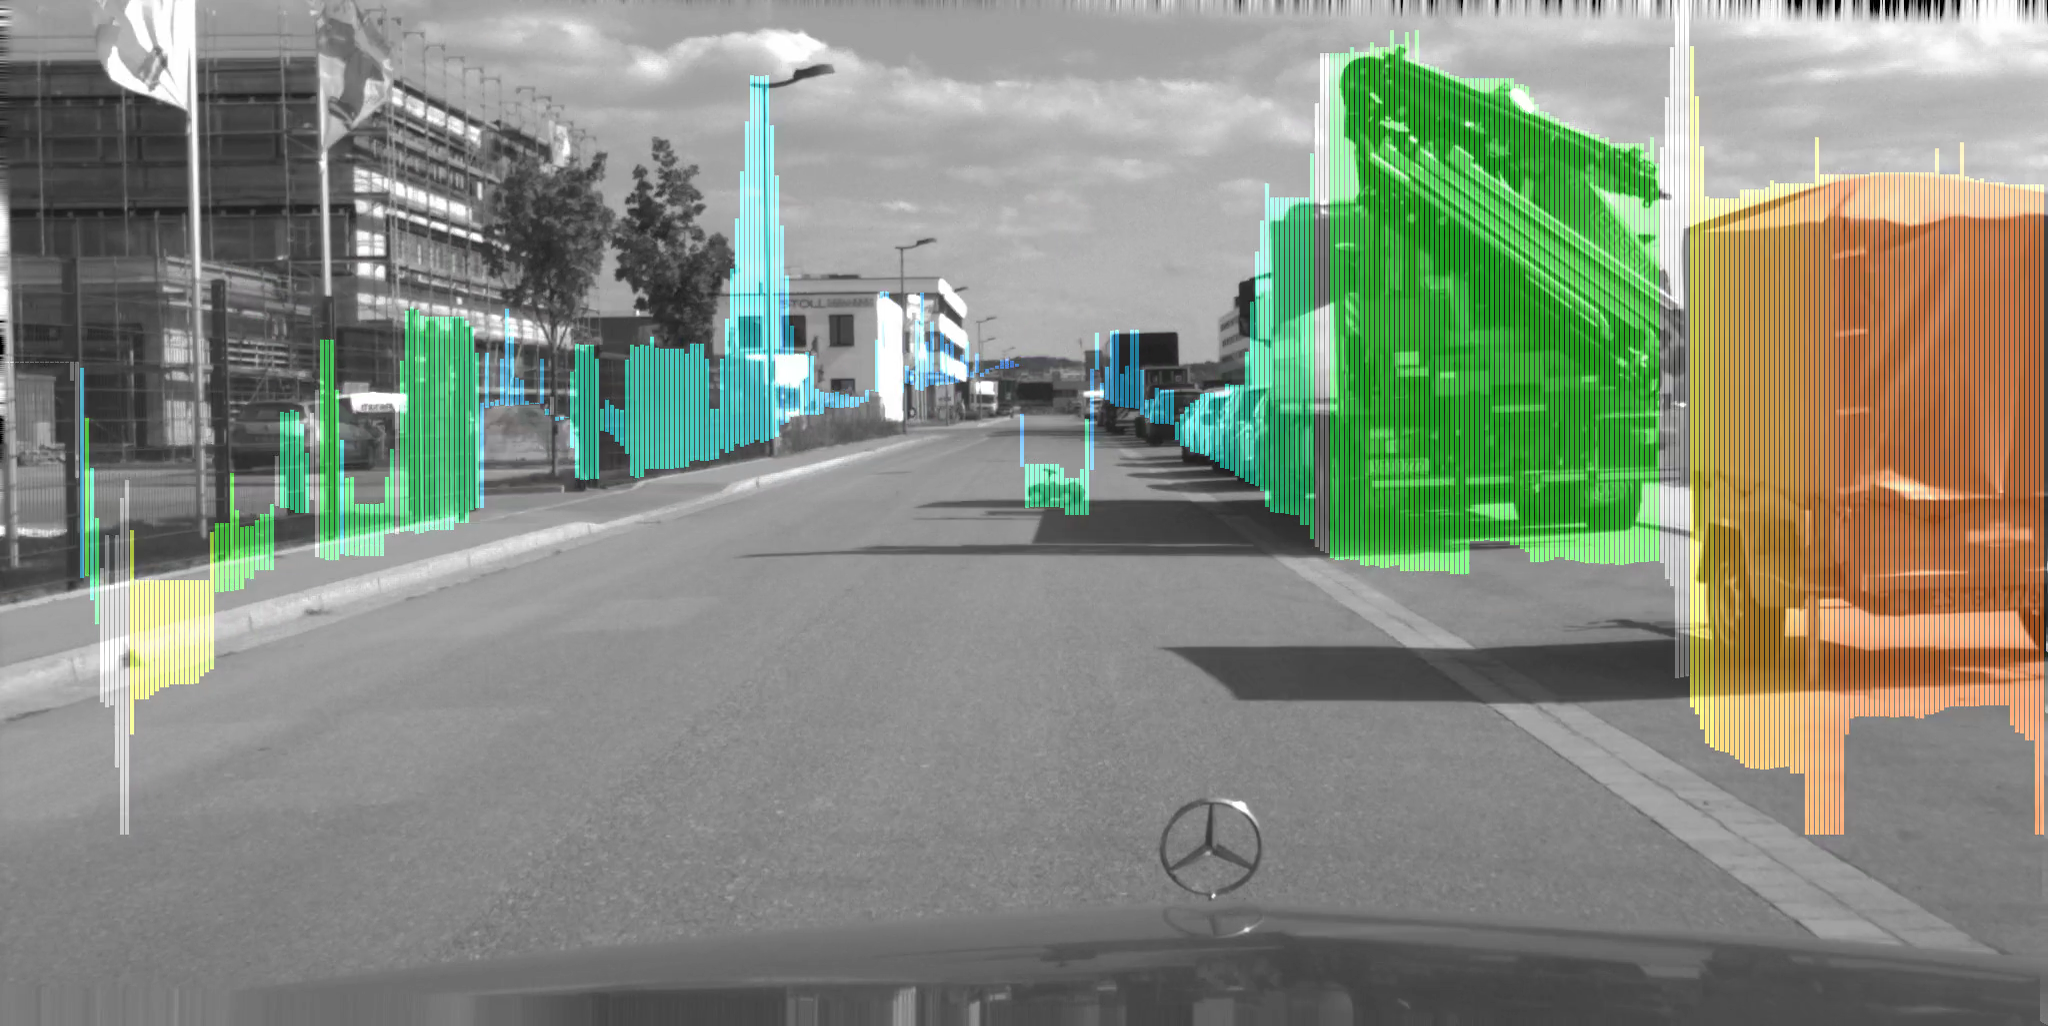
\includegraphics[width=\textwidth]{small_object.png}
\caption{Сегментация изображения согласно модели Stixel World. Цветом закодировано расстояние.}
\label{fig:stix_small}
\end{figure}

\begin{figure}[H]
\centering
\includegraphics[width=\textwidth]{offroad.png}
\caption{Выделение области, безопасной для движения, с помощью сегментации согласно модели Stixel World.}
\label{fig:stix_offroad}
\end{figure}






\newpage
\section{Алгоритм детектирования маркеров дорожной разметки}

На основе алгоритме из статьи \cite{aly2008real} нами был разработан алгоритм детектирования маркеров дорожной разметки. Данный алгоритм рассчитан на поиск маркеров дорожной разметки в виде прямых линий. Алгоритм включает в себя защиту от ложных срабатываний на некоторых дополнительных элементах разметки: пешеходный переход, остановка общественного транспорта, маркеры направлений движения. Кроме того, с помощью разработанного алгоритма возможно детектировать, например, бордюр, что необходимо в условиях движения в условиях города.

Псевдокод разработанного алгоритма представлен в листинге \ref{alg:markers}.

\begin{algorithm}
\caption{Выделение маркеров дорожной разметки на изображении}\label{alg:euclid}
\label{alg:markers}
\begin{algorithmic}[1]
\Require цветное изображение $img$, калибровочные данные для камеры
\Ensure Маска для изображения $img$, на которой отличные от нуля значения соответствуют маркерам дорожной разметки
\State Применить к $img$ преобразование Bird's Eye View
\State Преобразовать изображение в пространство HSV и извлечь канал Value, обозначим это новое изображение $imgHsvValue$
\State Применить морфологическое размыкание к изображению $imgHsvValue$ для удаления недостаточно тонких линий
\State Вычислить в каждой точке $imgHsvValue$ значение горизонтального оператора Собеля, обозначим получившееся изображение $imgSobel$
\State На $imgSobel$ приравнять к нулю все точки, направление градиента в которых существенно отличается от горизонтального
\State Разбить $imgSobel$ на непересекающиеся прямоугольники одинакового размера, обозначим каждый такой прямоугольник $Rect(i, j)$
\ForAll{$(i, j)$}
\State Пометим $Rect(i, j)$ как содержащий разметку, если сумма пикселей, попавших в этот прямоугольник больше порога
\EndFor
\State Интерпретируя центры $Rect(i, j)$ как точки на изображении, с помощью алгоритма RANSAC поочерёдно извлекаем все линии разметки
\end{algorithmic}
\end{algorithm}

Отметим, что отсутствие срабатываний на пешеходных переходах и на маркерах направлений движения достигается за счёт строки 3 листинга, а отсутствие срабатываний на остановках общественного транспорта достигается за счёт строки 5.

Кроме того, на рис. \ref{fig:lanes_pipline} изображены промежуточные результаты алгоритма. Слева направо на изображении представлены результаты после шагов 5, 9, 10. 

\begin{figure}[H]
     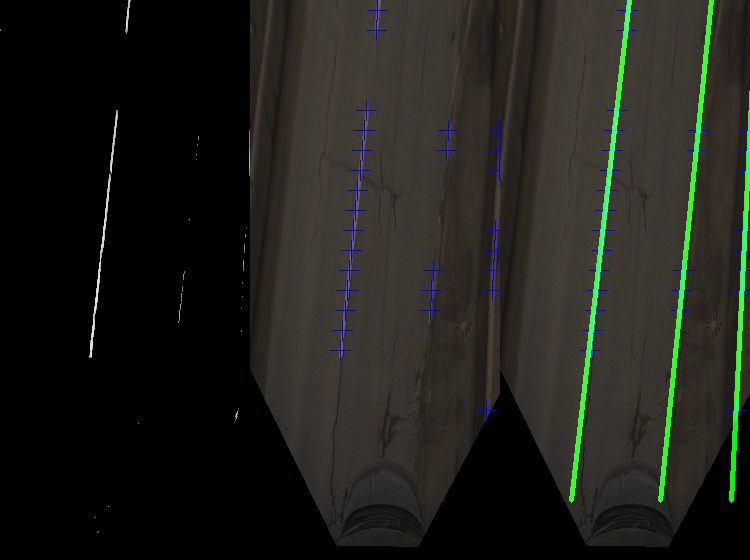
\includegraphics[width=\textwidth]{lanes_pipeline.png}
     \caption{Пример работы алгоритма выделения маркеров дорожной разметки}
     \label{fig:lanes_pipline}
\end{figure}


\newpage
\section{Апробация}

\subsection{Данные}

Для оценки качества работы алгоритма детектирования препятствий, были выбраны следующие наборы данных.
\begin{itemize}
\item Тестовый набор для алгоритмов детектирования объектов KITTI \cite{Geiger2012CVPR}.
\item Тестовый набор для алгоритмов детектирования объектов Lost and Found \cite{pinggera2016lost}.
\end{itemize}

Набор данных KITTI состоит из приблизительно 8000 изображений, полученных с помощью стереокамеры, установленной на крыше автомобиля. Изображения были получены в рамках движения автомобиля по дорогам общего пользования Германии. Каждое изображение проаннотировано прямоугольниками, описанными вокруг объектов из следующих классов: велосипедист, пешеход и автомобиль.

\textbf{\Large \color{Red} TODO}

\subsection{Оценка качества работы алгоритмов}

\subsubsection{Методика оценки алгоритма детектирования препятствий}

Так как выбранные наборы данных содержат аннотацию в виде описывающих прямоугольников, было решено применить следующий подход оценки. 
\begin{enumerate}
\item На изображении оцениваются параметры модели Stixel World.
\item Для каждого описывающего прямоугольника из аннотации из всех стикселей выбираются те, горизонтальная координата которых заключена между левой и правой границей прямоугольника.
\item Для выбранных стикселей вычисляется медиана нижней границы.
\item Отличие вычисленной медианы от нижней границы описывающего прямоугольника из аннотации принимается метрикой качества для данного изображения.
\item Метрики качества аггрегируются для всей коллекции.
\end{enumerate}

\textbf{\Large \color{Red} TODO}

\subsubsection{Результаты оценки алгоритма детектирования препятствий}

\textbf{\Large \color{Red} TODO}

\subsubsection{Сравнение результатов с реализацией модели Stixel World без использования карт диспаритета}

\textbf{\Large \color{Red} TODO}

\newpage
\section{Заключение}

В рамках данной работы были достигнуты следующие результаты.

\begin{itemize}
\item На основе подхода Stixel World и классического стереозрения разработан и релизован на языке C++ прототип алгоритма решения задачи поиска препятствий движению автомобиля на видеопоследовательности, полученной со стереокамеры, закреплённой на лобовом стекле автомобиля.

\item На основе методов классической обработки изображений разработан и реализован на языке Python прототип алгоритма поиска маркеров дорожной разметки на изображении, полученном с камеры, закреплённой на лобовом стекле автомобиля.

\item Выполнена апробация разработанных алгоритмов на наборах данных KITTI и tuSimple, а также на собственных данных.

\end{itemize}

\newpage

\bibliographystyle{ugost2008ls}
\bibliography{diploma.bib}
\end{document}


